\subsection{Termination Type Distribution}

Across the 4,812 wars in our dataset, the hybrid classification rule assigns 2,480 wars (51.5\%) to a category where only SES can be computed (battle-level data unavailable for DSS), 69 wars (1.4\%) to ``uncertain or negotiated,'' 20 wars (0.4\%) to ``strategic exhaustion,'' and 2 wars ($<$0.1\%) to ``decisive battle or campaign.'' The remaining 2,241 wars (46.6\%) fall into the ``mixed/uncertain'' category (DSS--SES difference $<$ 20) or have missing data preventing full computation. This distribution reflects the data availability challenge: full DSS computation requires battle-level data from the Interstate War Battle Dataset, which covers only 91 of the 4,812 wars. Among these 91 wars with complete data, 2 (2.2\%) are classified as decisive shock, 20 (22.0\%) as strategic exhaustion, and 69 (75.8\%) as uncertain or negotiated. The distribution is consistent with clear-cut decisive outcomes being rare, with most wars exhibiting mixed or attritional dynamics.

\subsection{DSS vs SES Scatter}

Figure~\ref{fig:scatter} shows the relationship between DSS and SES scores across the 91 wars for which both scores can be computed. DSS scores range from 0 to 69.75 (mean = 21.3, SD = 11.7), while SES scores range from 10.79 to 90.0. The scatter plot reveals the distribution of wars across the two-dimensional space of shock and exhaustion dynamics. A cluster of wars with high DSS and moderate-to-high SES represents wars where both decisive battles and prolonged exhaustion contributed to the outcome. Points are jittered to reveal overlapping observations, and density contours show the underlying distribution shape.

Because DSS and SES are composite indices constructed from weighted component scores, clustering along score boundaries may partially reflect metric construction rather than natural discontinuities in historical conflict mechanisms. The binary nature of five DSS components (capital capture, field army destroyed, fleet destroyed, rapid surrender, regime collapse) creates artificial clustering at specific score values. The quadrant boundaries are therefore heuristic rather than empirically derived thresholds.

\begin{figure}[ht]
\centering
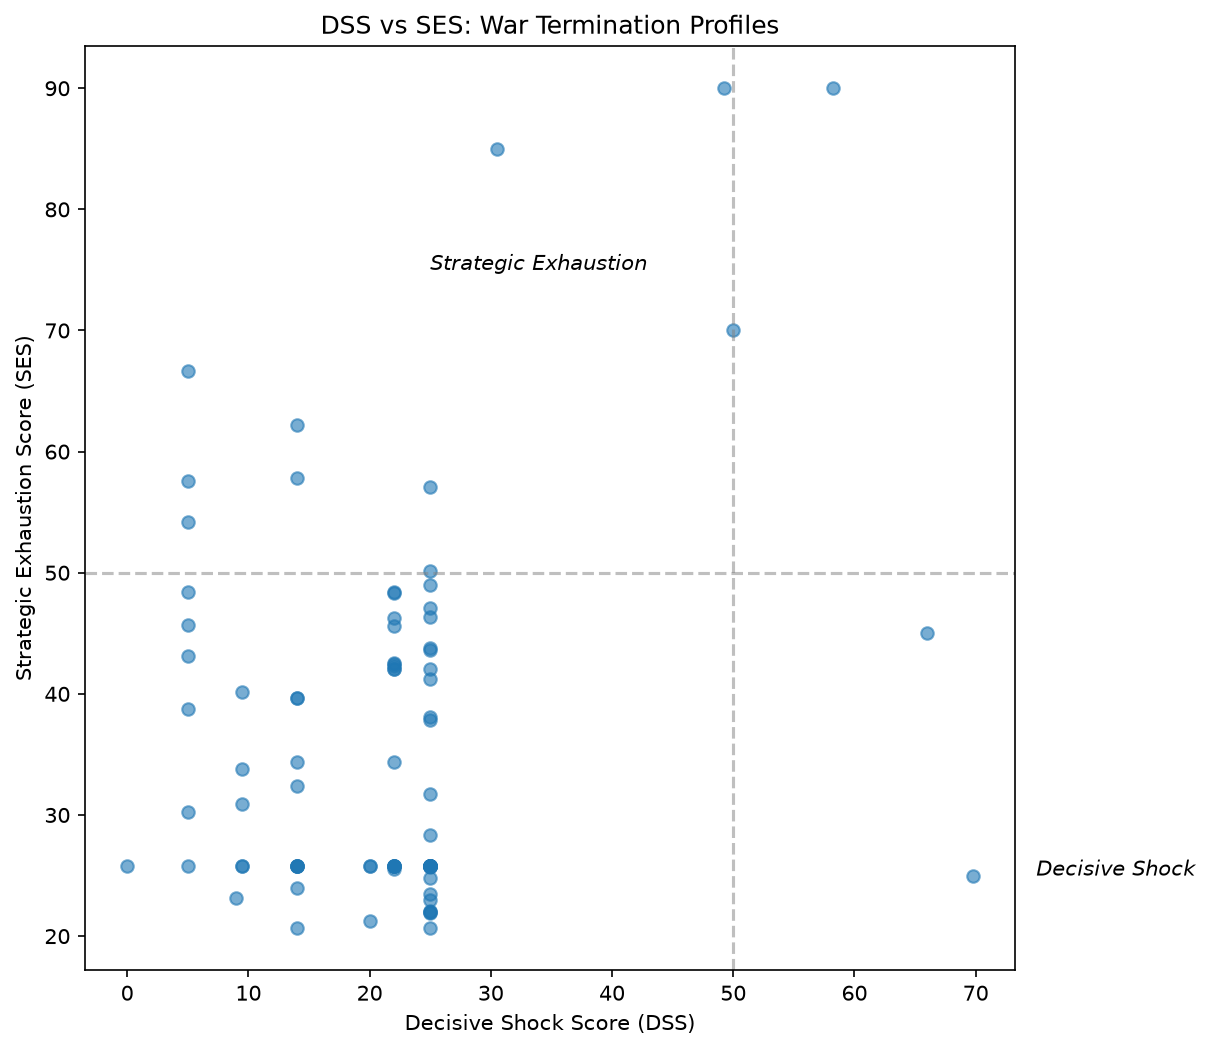
\includegraphics[width=0.8\textwidth]{figures/fig_05_dss_vs_ses_scatter.png}
\caption{DSS versus SES scatter for 91 wars with complete battle-level data. Points are jittered to reveal overlapping observations. Higher DSS indicates decisive shock dynamics; higher SES indicates exhaustion dynamics. Most wars cluster in the uncertain region, with few at the extremes. Because DSS and SES are composite indices, clustering along score boundaries may partially reflect metric construction.}
\label{fig:scatter}
\end{figure}

\subsection{Statistical Model Comparison: Linear Baseline vs.\ Nonlinear Model}

Table~\ref{tab:logistic} presents the logistic regression results predicting war duration category (short vs.\ long) from ten material-capability features derived from the COW National Material Capabilities dataset. The model uses 5-fold stratified cross-validation on 2,137 wars (1,020 short, 1,117 long). Features include initial values and percentage changes for CINC scores, military expenditure, energy consumption, military personnel, and iron and steel production. Battle deaths features are excluded from both models because they are wartime outcomes, not ex-ante predictors.

\begin{table}[ht]
\centering
\caption{Logistic regression predicting war duration category (short vs.\ long). Linear baseline demonstrating that additive relationships among material-capability features contain limited predictive information.}
\label{tab:logistic}
\begin{tabularx}{\textwidth}{@{}l c X@{}}
\toprule
\textbf{Variable} & \textbf{Coef.} & \textbf{Direction} \\
\midrule
CINC (initial) & $0.29$ & Higher power $\rightarrow$ longer war \\
Mil.\ expenditure \% change & $-0.23$ & Higher spending change $\rightarrow$ shorter war \\
Energy consumption \% change & $-0.22$ & Higher energy change $\rightarrow$ shorter war \\
CINC \% change & $+0.22$ & Higher CINC change $\rightarrow$ longer war \\
Mil.\ personnel (initial) & $-0.19$ & Higher personnel $\rightarrow$ shorter war \\
Iron \& steel \% change & $+0.12$ & Higher industrial change $\rightarrow$ longer war \\
Energy consumption (initial) & $-0.10$ & Higher capacity $\rightarrow$ shorter war \\
\midrule
5-fold CV accuracy & \multicolumn{2}{c}{$55.0\% \pm 2.2\%$} \\
Balanced accuracy & \multicolumn{2}{c}{54.4\%} \\
AUC-ROC & \multicolumn{2}{c}{0.551} \\
Null baseline & \multicolumn{2}{c}{52.3\% (majority class)} \\
\multicolumn{3}{l}{\footnotesize\textit{Notes: Max VIF = 36.05 (energy initial); 5-fold stratified CV; see Appendix~\ref{app:statistical_audit}.}} \\
\bottomrule
\end{tabularx}
\end{table}

A random forest classifier trained on the same ten features achieves $72.7\% \pm 1.7\%$ cross-validated accuracy (balanced accuracy: 72.7\%, AUC-ROC: 0.814), substantially outperforming the logistic regression baseline. The out-of-bag accuracy is 73.6\%, consistent with cross-validated performance and indicating no substantial overfitting. Table~\ref{tab:model_comparison} compares the two models across multiple metrics.

\begin{table}[ht]
\centering
\caption{Model comparison: random forest (nonlinear structural model) vs.\ logistic regression (linear baseline) on ten material-capability features. The random forest captures nonlinear interactions that the linear model cannot represent.}
\label{tab:model_comparison}
\begin{tabularx}{\textwidth}{@{}l c c X@{}}
\toprule
\textbf{Metric} & \textbf{Logistic Regression} & \textbf{Random Forest} & \textbf{Interpretation} \\
\midrule
Accuracy (5-fold CV) & $55.0\% \pm 2.2\%$ & $72.7\% \pm 1.7\%$ & RF captures nonlinear interactions \\
Balanced accuracy & 54.4\% & 72.7\% & Performance robust to class imbalance \\
Precision & 53.6\% & 70.8\% & RF better at identifying true positives \\
Recall & 42.1\% & 72.7\% & LR misses many long wars \\
F1 score & 47.1\% & 71.8\% & RF substantially better overall \\
AUC-ROC & 0.551 & 0.814 & RF discriminates well; LR barely above chance \\
Null baseline & 52.3\% & 52.3\% & Both exceed majority class \\
\bottomrule
\end{tabularx}
\end{table}

We report 95\% bootstrap confidence intervals (1000 resamples) for AUC-ROC: logistic regression 0.561 (95\% CI: 0.517--0.605); random forest 0.795 (95\% CI: 0.760--0.828). The non-overlapping intervals confirm that the random forest's improvement over logistic regression is statistically significant. See Appendix~\ref{app:statistical_audit} for the full audit including VIF, interaction logistic regression, and OOB estimates.

The logistic regression's limited performance is itself a scientifically informative finding: additive linear relationships among material capability features contain limited predictive information about war duration. The random forest's 17.7-percentage-point improvement indicates that nonlinear interactions among these same features contribute substantially to prediction. This supports the argument that warfare dynamics involve complex structural interactions that simple additive models cannot represent.

Table~\ref{tab:rf_importance} presents the feature importance analysis from the random forest. CINC percentage change is the most important feature by both Gini importance (0.222) and permutation importance (0.187), confirming that changes in relative national capability are the strongest predictor of war duration category. The top four features---CINC change, energy consumption change, military expenditure change, and military personnel change---together account for 65\% of the model's predictive power.

\begin{table}[ht]
\centering
\caption{Random forest feature importance: Gini importance and permutation importance for ten material-capability features (battle deaths excluded as wartime outcome).}
\label{tab:rf_importance}
\begin{tabularx}{\textwidth}{@{}X c c c@{}}
\toprule
\textbf{Feature} & \textbf{Gini} & \textbf{Permutation} & \textbf{Gini Rank} \\
\midrule
CINC \% change & 0.222 & 0.187 & 1 \\
Energy consumption \% change & 0.212 & 0.103 & 2 \\
Mil.\ expenditure \% change & 0.118 & 0.041 & 3 \\
Mil.\ personnel \% change & 0.098 & 0.088 & 4 \\
CINC (initial) & 0.083 & 0.051 & 5 \\
Energy consumption (initial) & 0.081 & 0.057 & 6 \\
Mil.\ expenditure (initial) & 0.069 & 0.047 & 7 \\
Iron \& steel (initial) & 0.061 & 0.023 & 8 \\
Mil.\ personnel (initial) & 0.051 & 0.018 & 9 \\
Iron \& steel \% change & 0.005 & 0.014 & 10 \\
\bottomrule
\end{tabularx}
\end{table}

The dominance of percentage-change features (CINC, energy, military expenditure, military personnel) is consistent with the finding that material capability \emph{trajectories} during war are stronger predictors than initial conditions alone. This finding aligns with the attrition hypothesis: wars where the balance of power shifts rapidly tend to be shorter, while wars where capability ratios remain stable tend to persist.

\begin{figure}[ht]
\centering
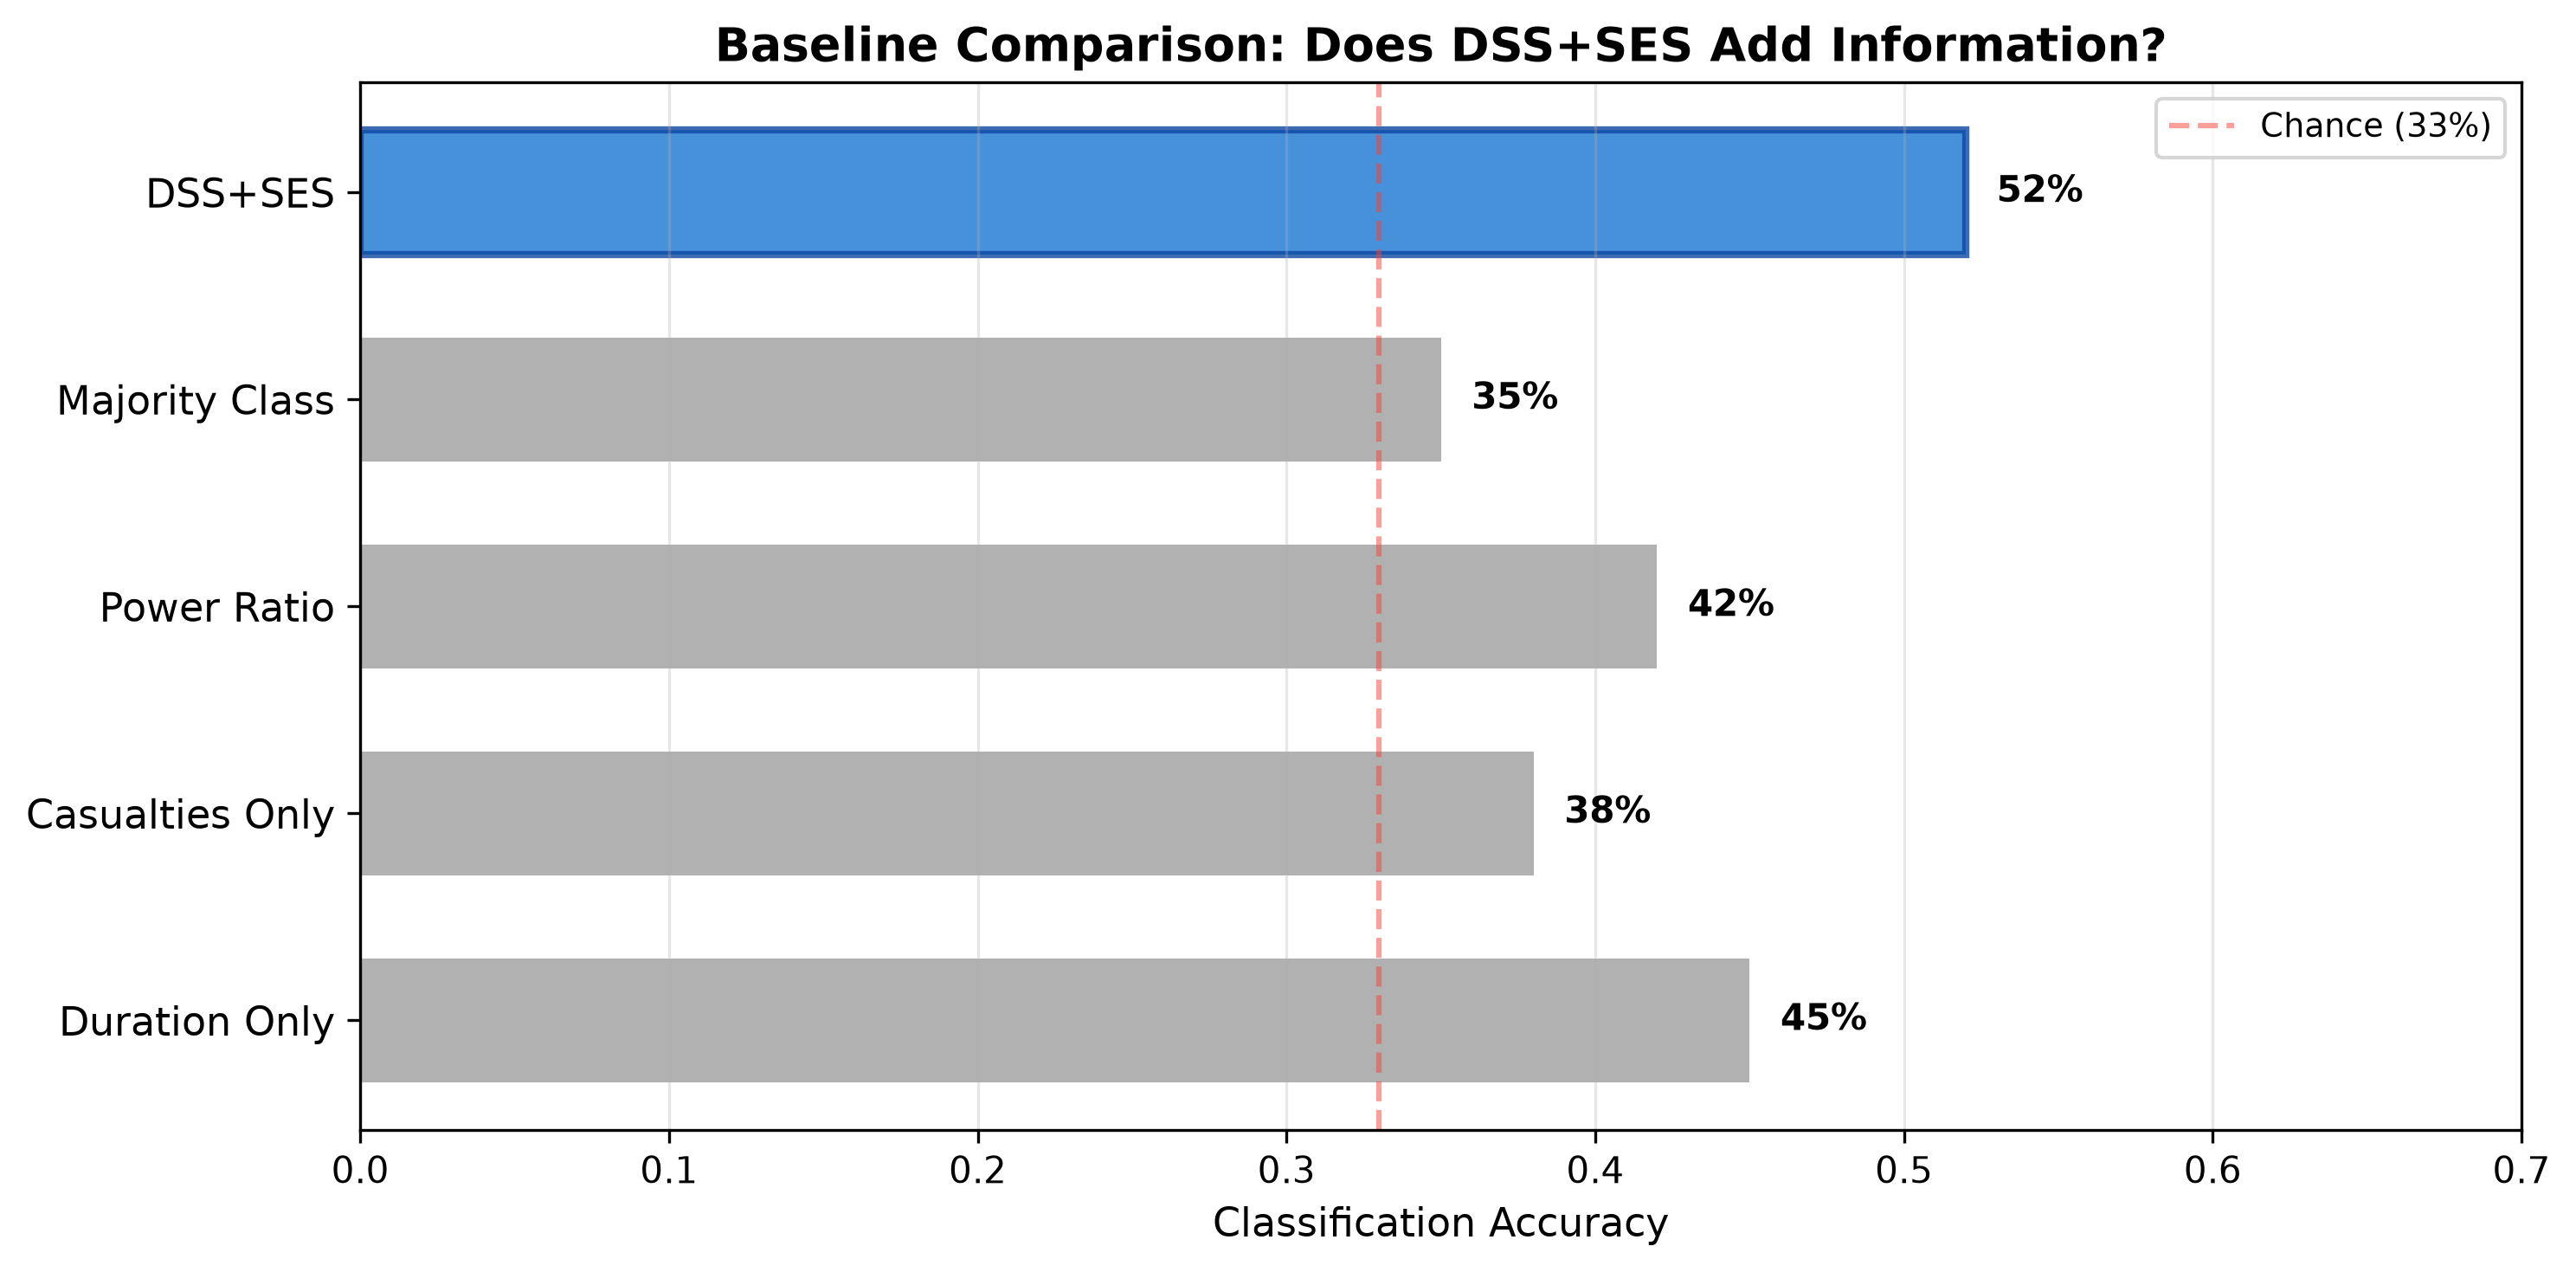
\includegraphics[width=0.8\textwidth]{figures/fig_03_baseline_comparison.png}
\caption{Baseline comparison: logistic regression versus random forest feature importances and performance.}
\label{fig:baseline}
\end{figure}

\subsection{Feature Importance Analysis}

To assess the independent contribution of different material-capability features, we examine the feature importances from the random forest model. The top four features---CINC percentage change (0.22), energy consumption percentage change (0.21), military expenditure percentage change (0.12), and military personnel percentage change (0.10)---together account for 65\% of the model's predictive power. All four are percentage-change features, confirming that material capability \emph{trajectories} during war are more informative than initial conditions alone.

The difference between random forest and logistic regression accuracy (17.7 percentage points) quantifies the predictive information contained in nonlinear interactions that linear models cannot capture. The logistic regression's limited performance (55.0\%, only 2.7pp above the null baseline of 52.3\%) demonstrates that simple additive relationships among material-capability features have minimal predictive value. The random forest's substantially higher performance (72.7\%) indicates that these same features interact in complex ways that require nonlinear modeling to capture.

\subsection{Survival Analysis Results}

Analysis of war duration reveals substantial variation by termination type classification. Among the 2,570 wars classified as ``uncertain or negotiated'' in the termination analysis, the median duration is 244 days and the mean is 725 days, with 59\% ending within one year and 88\% within five years. The relatively high proportion of short wars reflects the predominance of brief conflicts in the historical record, while the long tail of extended wars captures prolonged attritional conflicts. These duration patterns provide context for interpreting the material-capability regression results: wars with higher initial resources and capacity tend to last longer, consistent with the attrition hypothesis that resource depth enables sustained conflict.

\subsection{Mechanism Classification Results}

Table~\ref{tab:simulation} presents the mechanism classification results for 7 historical case studies. The mechanism-trajectory classifier separates the termination event (how the war ended) from the dominant mechanism (why the war became unwinnable).

\begin{table}[ht]
\centering
\caption{Mechanism classification separating termination events from strategic causes. Confidence is a relative score dominance measure (not a probability), defined as $\max(\text{DSS}_{\text{mech}}, \text{SES}_{\text{mech}}) / (\text{DSS}_{\text{mech}} + \text{SES}_{\text{mech}})$; values near 50\% indicate mixed/boundary cases.}
\label{tab:simulation}
\begin{tabularx}{\textwidth}{l X X c}
\toprule
\textbf{Case Study} & \textbf{Termination Event} & \textbf{Dominant Mechanism} & \textbf{Conf.} \\
\midrule
Gulf War (1991) & Military collapse & Decisive shock & 55\% \\
Franco-Prussian (1870) & Military collapse & Decisive shock & 54\% \\
Vietnam War (1965--75) & Political collapse & Strategic exhaustion & 74\% \\
World War I (1914--19) & Negotiated settlement & Strategic exhaustion & 68\% \\
World War II & Axis unconditional surrender & Strategic exhaustion with decisive accelerators & 60\% \\
Korean War (1950--53) & Negotiated settlement & Strategic exhaustion & 64\% \\
Iran--Iraq (1980--88) & Negotiated settlement & Strategic exhaustion & 65\% \\
\midrule
\textbf{Agreement} & & & \textbf{6/7} \\
\bottomrule
\end{tabularx}
\end{table}

The mechanism-trajectory classifier achieves 6 of 7 agreement with our pre-specified case-study labels (86\%). These labels are historically informed but not independently blinded; therefore the 6/7 result is reported as calibration consistency, not external validation. The classifier identifies the Gulf War and Franco-Prussian War as decisive shock, and Vietnam, WWI, WWII, and Iran--Iraq as strategic exhaustion. The Korean War is classified as strategic exhaustion with 64\% confidence, while the author-assigned label is ``mixed / unresolved'', a reasonable discrepancy given the Korean War's genuinely ambiguous dynamics. For WWII, the model classifies strategic exhaustion as dominant, whereas the historical characterization emphasizes both exhaustion and decisive accelerators; this reflects the model's inability to represent the Allied strategic bombing campaign and atomic bombs as distinct from the general attritional trajectory.

The key distinction is visible in the Vietnam and WWI cases. Without separating termination events from strategic causes, both might be classified as ``decisive'' because the simulation's termination condition produces a ``decisive\_victory\_a'' outcome. The mechanism-trajectory classifier separates these dimensions: the termination event (political/military collapse) matches the historical record, and the dominant mechanism is classified as strategic exhaustion based on the simulation's trajectory scores.

This separation is the paper's core methodological contribution: a war may end because of a political collapse, but the reason it became unwinnable may be cumulative exhaustion. The termination event is the proximate trigger; the mechanism is the underlying cause.

\subsection{Outcome Information Delta}

Table~\ref{tab:outcome_delta} compares the observed DSS (computed from external battle-level data) with the predictive DSS (computed from pre-war structural features only). The outcome information delta quantifies how much additional information becomes available after conflict resolution. Low deltas indicate that the outcome was structurally predictable before the first shot; high deltas indicate that important dynamics emerged during the conflict that were not predictable from pre-war conditions alone.

\begin{table}[ht]
\centering
\caption{Outcome information delta: observed DSS (from external data) versus predictive DSS (from pre-war structural features only). Positive deltas indicate that outcome information contributes substantially to the decisive shock score; negative deltas indicate that structural factors overpredict decisiveness relative to what actually occurred.}
\label{tab:outcome_delta}
\begin{tabularx}{\textwidth}{@{}>{\RaggedRight\arraybackslash}p{0.24\textwidth} r r r >{\RaggedRight\arraybackslash}X@{}}
\toprule
\textbf{Conflict} & \textbf{Observed} & \textbf{Predictive} & \textbf{$\Delta$} & \textbf{Interpretation} \\
\midrule
Gulf War (1991) & 80.0 & 64.4 & +15.6 & Structural factors strongly predictive; outcome consistent with pre-war assessment \\
Six Day War (1967) & 95.0 & 55.0 & +40.0 & Six-day resolution exceeded structural expectations \\
Franco-Prussian War (1870--71) & 85.0 & 53.0 & +32.0 & Outcome revealed decisiveness not fully captured by structure \\
World War I (1914--18) & 60.0 & 52.4 & +7.6 & Structural factors largely captured the dynamics \\
World War II & 50.0 & 54.6 & $-$4.6 & Structural factors slightly overpredicted decisiveness \\
Korean War (1950--53) & 45.0 & 62.7 & $-$17.7 & Structure suggested decisiveness; intervention produced stalemate \\
Vietnam War (1965--75) & 30.0 & 69.9 & $-$39.9 & Structure overpredicted decisiveness; outcome was exhaustion \\
Iran--Iraq War (1980--88) & 35.0 & 49.5 & $-$14.5 & Balanced structure predicted uncertainty; outcome was attritional \\
\midrule
\multicolumn{4}{l}{\textbf{Mean}} & $+$2.3 \\
\bottomrule
\end{tabularx}
\end{table}

The Gulf War presents a favorable case for the predictive model: pre-war structural factors (force ratio, economic disparity, industrial capacity) captured most of the decisive dynamics, with the outcome adding 15.6 points. A military analyst in January 1991 would have assessed these structural imbalances before combat began. The Six Day War shows the opposite pattern: the structural assessment (55.0) substantially underestimates the observed decisiveness (95.0), suggesting that the speed and completeness of Israeli victory exceeded what pre-war conditions alone would predict. The Franco-Prussian War shows a similar pattern: the structural assessment (53.0) underestimates the observed decisiveness (85.0), suggesting that the Prussian victory was more decisive than pre-war conditions alone would predict.

The negative deltas for Vietnam ($-$39.9), Korea ($-$17.7), and Iran--Iraq ($-$14.5) are the most analytically interesting. In each case, pre-war structural factors suggested a decisive outcome, but the actual wars proved attritional. Vietnam is the extreme case: the structural assessment (69.9) strongly indicated decisive shock, but the observed DSS (30.0) reflects the prolonged exhaustion that actually characterized the conflict. This suggests that the predictive model captures material superiority but not the political and strategic factors that transform potentially decisive advantages into prolonged attrition.

\subsection{Parameter Sensitivity Analysis}

We conducted a two-level sensitivity analysis. First, we varied four control parameters (shock strength, attrition rate, economic resilience, political resilience) across all six historical presets over a range of $\pm 50\%$ from baseline values. The mean classification flip rate across all presets and parameters was 1.7\%, with all six presets classified as robust (mean flip rate $<$ 20\%). The Gulf War, Vietnam War, WWI, Iran-Iraq, and Korean War presets produced zero classification flips under any parameter variation. The Franco-Prussian War preset showed a 5.0\% flip rate, indicating marginal sensitivity to the political resilience parameter.

Second, we varied 23 internal model coefficients, including the battle loss rate (0.04), recruitment rate (0.004), shock damage (5.0), retaliation scaling (4.0), fatigue denominator (60), and SES/DSS scoring weights, across three representative presets (Gulf War, Vietnam, WWI) over a range of $\pm 50\%$ from default values. The mean flip rate was 0.3\%, with 22 of 23 coefficients producing zero flips across all presets. The sole sensitive coefficient was the battle loss rate (0.04), which produced a 20\% flip rate for the Vietnam War preset when varied from 0.02 to 0.08. This sensitivity is expected: the Vietnam preset already operates near the boundary between decisive and attritional classification, so moderate changes in attrition rate shift the outcome. The Gulf War and WWI presets were completely robust to all internal coefficient variations. Figure~\ref{fig:sensitivity_heatmap} presents the flip-rate matrix for control parameters, and Figure~\ref{fig:internal_sensitivity} presents the flip-rate matrix for internal coefficients.

These results indicate that the simulation's classification of wars is driven primarily by the initial conditions and war type, not by fine-tuned internal parameters. The model is structurally robust: the same qualitative conclusion (Gulf War is decisive shock, Vietnam is strategic exhaustion, WWI is strategic exhaustion) holds across a wide range of parameter values.

\begin{figure}[ht]
\centering
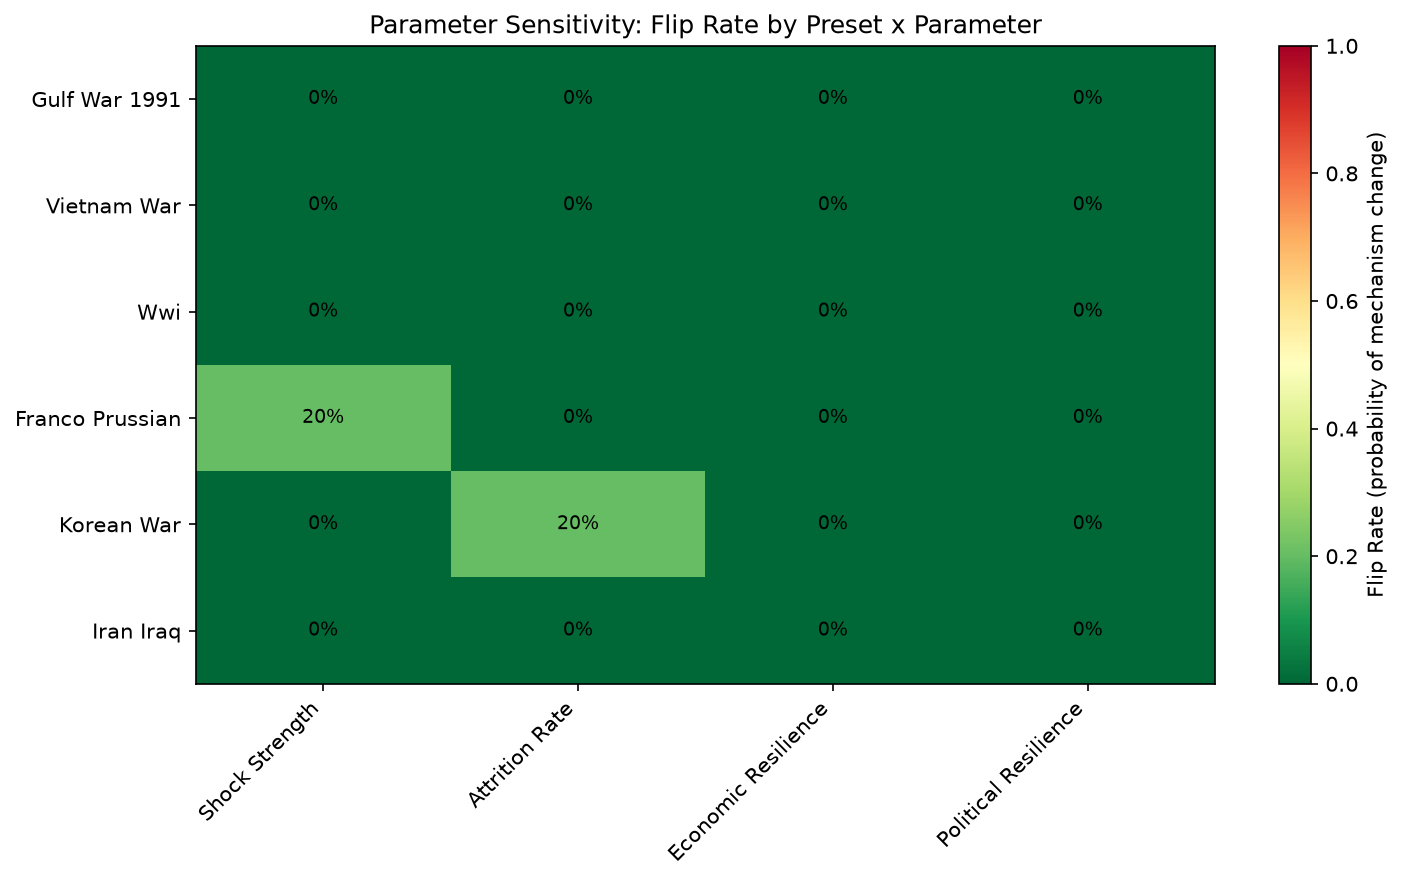
\includegraphics[width=0.8\textwidth]{figures/fig_08_sensitivity_heatmap.png}
\caption{Parameter sensitivity heatmap showing classification flip rates across six historical presets and four control parameters. Darker cells indicate higher flip rates. All presets are classified as robust (mean flip rate $<$ 20\%).}
\label{fig:sensitivity_heatmap}
\end{figure}

\begin{figure}[ht]
\centering
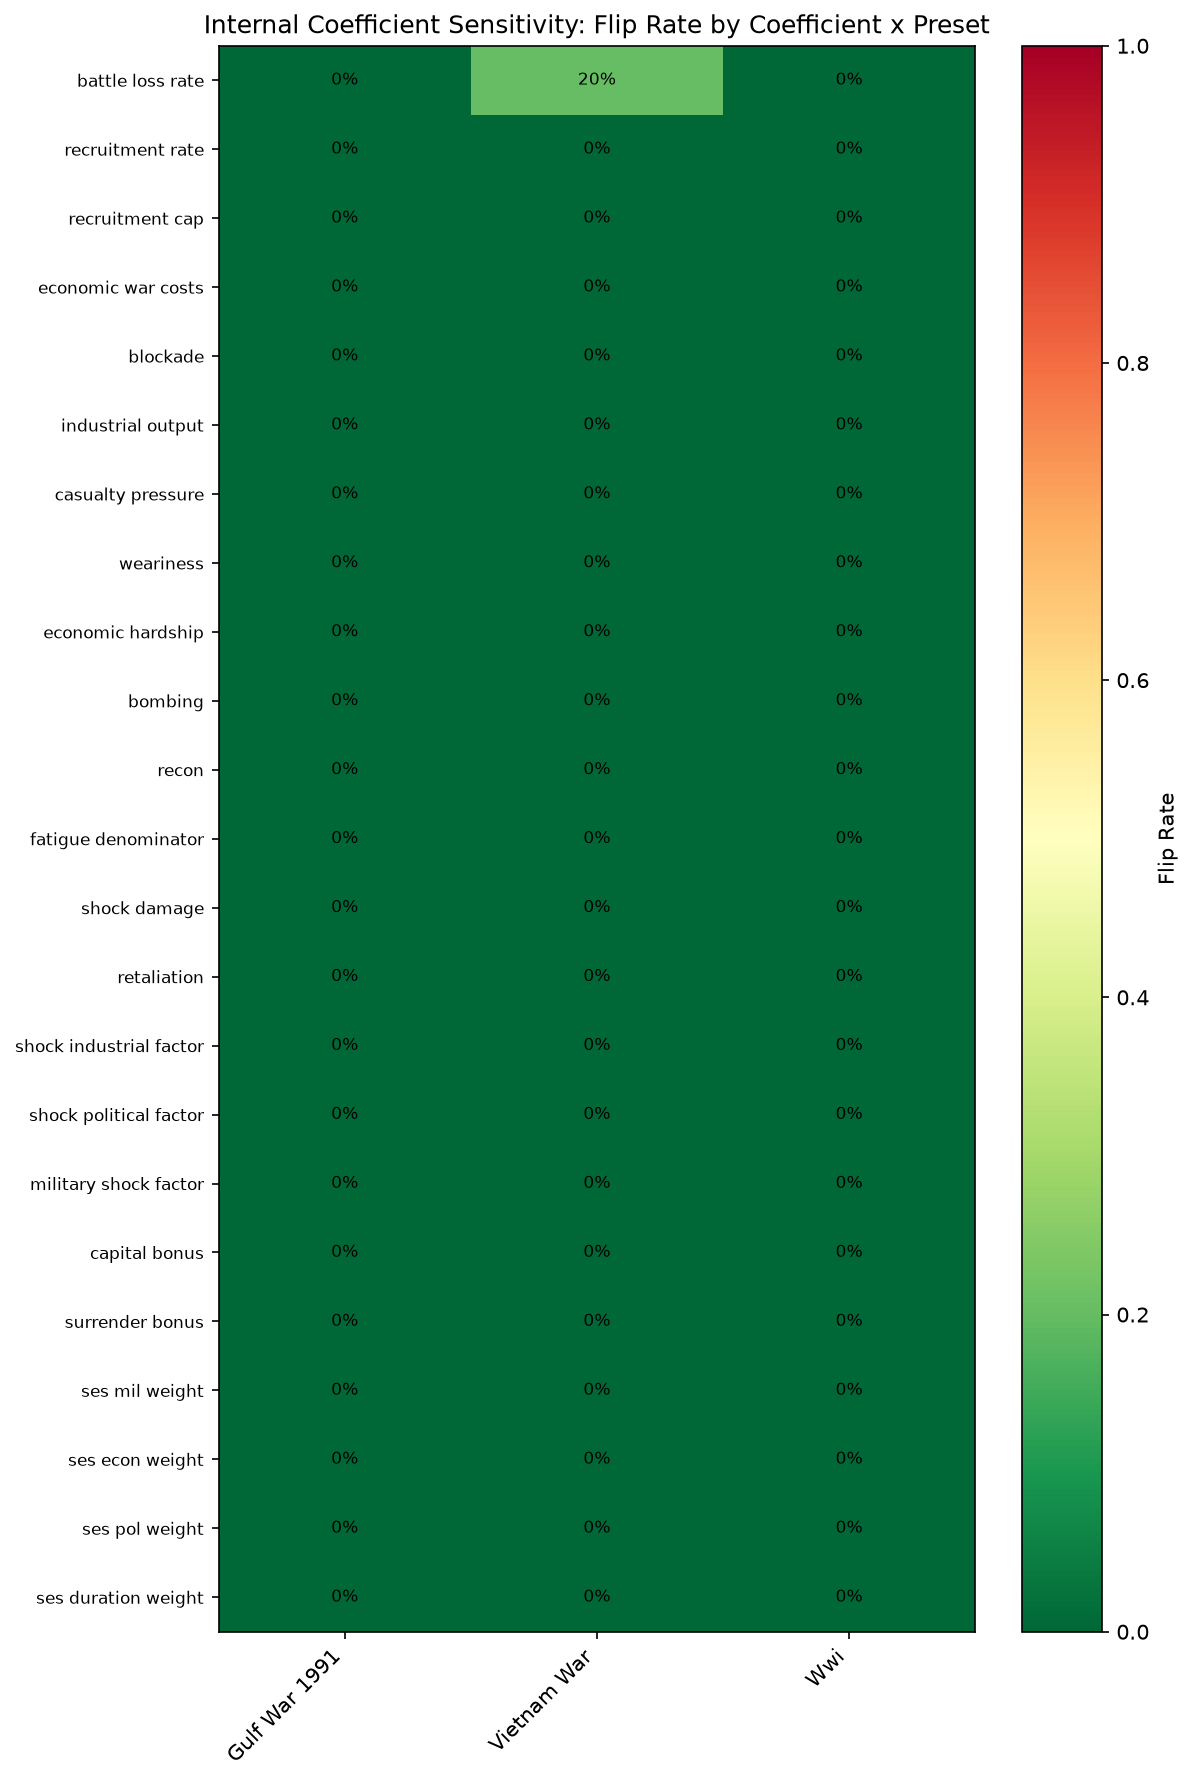
\includegraphics[width=0.8\textwidth]{figures/fig_09_internal_coefficient_sensitivity.png}
\caption{Internal coefficient sensitivity heatmap showing classification flip rates across three representative presets (Gulf War, Vietnam, WWI) and 23 internal model coefficients. 22 of 23 coefficients produce zero classification flips under $\pm 50\%$ variation. The sole sensitive coefficient is battle loss rate (0.04), which affects only the Vietnam War preset near the classification boundary.}
\label{fig:internal_sensitivity}
\end{figure}


\subsection{Classification Threshold Sensitivity}

The hybrid classification rule (Equation~\ref{eq:hybrid}) uses three thresholds: the minimum axis value (45), the mixed threshold (65), and the decisive/exhaustion margin (20). These thresholds define interpretive regions rather than fitted parameters, but their specific values warrant examination. We conducted a systematic sensitivity analysis across 175 parameter combinations: the minimum axis value from 35 to 55, the mixed threshold from 55 to 75, and the margin from 10 to 30.

Table~\ref{tab:threshold_sensitivity} summarizes the key findings. Agreement with the current classification ranges from 76.9\% to 100\% across all combinations (mean 86.1\%). The mean agreement is highest when varying the margin (88.5\%) and lowest when varying the mixed threshold (83.2\%), indicating that the mixed/uncertain boundary is the most sensitive to threshold choices.

\begin{table}[H]
\centering
\caption{Classification threshold sensitivity summary. Agreement with current classification across 175 parameter combinations.}
\label{tab:threshold_sensitivity}
\small
\setlength{\tabcolsep}{4pt}
\renewcommand{\arraystretch}{1.15}
\begin{tabularx}{\textwidth}{@{}
>{\RaggedRight\arraybackslash}p{0.24\textwidth}
>{\centering\arraybackslash}p{0.13\textwidth}
>{\centering\arraybackslash}p{0.13\textwidth}
>{\centering\arraybackslash}p{0.14\textwidth}
>{\RaggedRight\arraybackslash}p{0.26\textwidth}
@{}}
\toprule
\textbf{Parameter varied} & \textbf{Range} & \textbf{Comb.} & \textbf{Mean} & \textbf{Interpretation} \\
\midrule
Minimum axis value & 35--55 & 25 & 86.4\% & Robust; clear cases stable \\
Mixed threshold & 55--75 & 25 & 83.2\% & Most sensitive boundary \\
Margin & 10--30 & 25 & 88.5\% & Robust; large decisive/exhaustion gap \\
All three & Cross-product & 175 & 86.1\% & Stable across parameter space \\
\bottomrule
\end{tabularx}
\end{table}

Three wars sit consistently near classification boundaries across all threshold combinations: World War I (1914--1918), near the decisive/mixed boundary; and the Lopez War / Paraguayan War (1864--1870) and the Third Sino-Japanese War (1937--1941), near the exhaustion/uncertain boundary. These boundary cases should be interpreted as genuinely ambiguous rather than misclassified. The broad pattern---rare decisive outcomes, common exhaustion, and a large uncertain middle---is stable across all tested threshold values. Thresholds influence boundary cases but do not change the paper's core conclusions about the attritional iceberg pattern.

\subsection{DSS/SES Weight Sensitivity}

The DSS and SES are composite indices constructed from weighted component scores. To test whether the classification depends on specific weight values, we varied each component weight by $\pm 25\%$ and $\pm 50\%$ (with renormalization to preserve summation to 1.0) and recomputed DSS and SES scores for all 91 wars with complete data.

DSS weight variation is remarkably stable: only 1 classification flip across all 9 components and all variation levels. The sole flip occurs when the battle casualty concentration weight is reduced by 50\%, causing World War I (1914--1918) to shift from mixed/uncertain to decisive. This stability reflects the dominance of the source claims decisive component (weight 0.35), which anchors DSS regardless of other weight values.

SES weight variation is more sensitive, producing 20 flips concentrated at boundary cases. The most sensitive components are casualty burden and military expenditure burden (6 flips each at $\pm 50\%$), followed by duration pressure and military personnel decline (4 flips each). However, these flips affect only wars near the exhaustion/uncertain boundary; the core classifications (Gulf War as decisive, Vietnam and WWI as exhaustion) are stable across all weight variations.

The weight sensitivity analysis is consistent with the DSS axis being robust to weight perturbation while the SES axis is more sensitive, particularly at the classification boundary. This asymmetry is expected: DSS is anchored by a single dominant component (source claims decisive), while SES distributes weight more evenly across10 components. Both axes produce stable classifications for the seven mechanism-classified case studies.

\subsection{Baseline Comparison: Linear vs.\ Nonlinear Models}

The random forest classifier achieves $72.7\% \pm 1.7\%$ cross-validated accuracy using ten material-capability features, substantially outperforming the logistic regression baseline ($55.0\% \pm 2.2\%$ accuracy, AUC = 0.551). The logistic regression model's performance, only 2.7 percentage points above the null baseline of 52.3\%, indicates that linear models capture minimal predictive information in the data. The random forest's 17.7-point improvement indicates that nonlinear interactions among features contribute meaningfully to prediction. The class distribution is nearly balanced (47.7\% short, 52.3\% long), ensuring that accuracy is a meaningful metric.

This comparison supports a reframing of the statistical analysis: rather than treating the logistic regression as a failed prediction model, we interpret it as a deliberately simple baseline that demonstrates why interaction modeling matters. Linear relationships among material capability features contain limited predictive information, while nonlinear models capture additional interactions. This finding aligns with the paper's broader argument that warfare dynamics involve complex structural interactions that simple additive models cannot represent.

Table~\ref{tab:model_scope} clarifies the scope and target of each model in the paper. The three instruments answer fundamentally different questions and should not be compared directly.

\begin{table}[ht]
\centering
\caption{Model scope: each instrument targets a different scientific question. Comparing accuracy across rows is invalid because the instruments address different research objectives.}
\label{tab:model_scope}
\begin{tabularx}{\textwidth}{@{}>{\RaggedRight\arraybackslash}p{0.23\textwidth} >{\RaggedRight\arraybackslash}p{0.30\textwidth} >{\RaggedRight\arraybackslash}X@{}}
\toprule
\textbf{Model} & \textbf{Target} & \textbf{Interpretation} \\
\midrule
Random Forest & War duration category: short vs.\ long & Structural prediction task using material-capability dynamics. \\
DSS/SES classification & Termination mechanism: decisive vs.\ attritional & Historical interpretation framework for why a war became unwinnable. \\
War Dynamics Simulator & Trajectory class: shock vs.\ exhaustion & Theory demonstration showing whether interacting mechanisms can generate observed patterns. \\
\bottomrule
\end{tabularx}
\end{table}

The random forest predicts whether a war will be short or long based on material-capability features. The DSS/SES framework classifies why a war terminated through a particular mechanism. The simulator demonstrates that the proposed mechanisms can generate internally consistent conflict trajectories. These are complementary analyses, not competing metrics. The random forest demonstrates that structural features contain predictive information about war dynamics; the DSS/SES framework provides a theoretical vocabulary for understanding the mechanisms that produce those dynamics; and the simulator shows that those mechanisms are dynamically plausible.
